\section{Projection sufficiency: when an epistemic abstraction loses the decision}

The preceding arguments show that particular scientific distinctions cannot be replaced by superficially similar quantities. There is a more general failure mode. A state abstraction may discard a coordinate that is necessary to determine which canonical update is licensed. Once two scientifically different worlds have been mapped to the same represented state, no downstream policy operating only on that state can reconstruct the lost distinction without additional observations.

Let \(S\) be a set of canonical scientific worlds, let
\[
\pi:S\longrightarrow Z
\]
be the state projection exposed to an update policy, and let
\[
a^*:S\longrightarrow\mathcal A
\]
be the registered correct canonical action, with \(\mathcal A\) containing actions such as hold, promote, restrict scope, revoke, supersede and cannot-check.

\begin{proposition}[Projection-collision impossibility]
If there exist \(x,y\in S\) with
\[
\pi(x)=\pi(y)
\qquad\text{but}\qquad
 a^*(x)\neq a^*(y),
\]
then no deterministic policy \(f:Z\to\mathcal A\) can be correct on both \(x\) and \(y\).
\end{proposition}

\begin{proof}
Because \(\pi(x)=\pi(y)=z\), a deterministic policy emits the same value \(f(z)\) in both worlds. Since the registered actions differ, that one value can equal at most one of \(a^*(x)\) and \(a^*(y)\).
\end{proof}

This proposition is intentionally independent of model intelligence. It does not say that an omitted fact can never be inferred from raw observations or external tools. It says that, once the policy interface is restricted to \(\pi(S)\), a distinction erased by \(\pi\) is unavailable to any deterministic downstream rule. The relevant question for an agent architecture is therefore not merely whether its state is convenient, but whether the state is a sufficient statistic for the scientific updates the architecture intends to govern.

\subsection{Minimal-twin projection audit}

We implemented a deterministic projection audit over 15 minimal-twin families corresponding to the adversarial failure classes used by the Paper~I evaluation programme. Each family contains two worlds that differ in exactly one registered scientific coordinate and require different canonical actions. All ordinary summary coordinates are held fixed inside the pair. The families include provenance strength, higher-order gluing, context/regime alignment, evidence independence, prediction versus mechanism, mechanism versus identification, workspace and experience non-authority, supersession, truth versus novelty, cannot-check, negative-history retention and legitimate promotion/supersession controls.

Seven state abstractions are compared at the representation level: text-memory summaries, provenance-only state, scalar confidence, pairwise compatibility, reviewer-vote state, a simple transactional state and the typed Orion authority projection. For each abstraction we partition the 30 worlds by the projected state. A projected bucket containing more than one required action is an information collision. The best possible deterministic classification accuracy available from that representation is then bounded by choosing the modal action in every projected bucket. We also calculate the maximum recall of legitimate canonical changes attainable with zero classification error: a promotion, restriction, revocation or supersession can be taken without risk only when every world sharing that projected state requires the same action.

\begin{table}[ht]
\centering
\footnotesize
\begin{tabular}{p{0.27\linewidth} >{\centering\arraybackslash}p{0.16\linewidth} >{\centering\arraybackslash}p{0.16\linewidth} >{\centering\arraybackslash}p{0.19\linewidth}}
\toprule
State projection & Identifiable accuracy & Unavoidable error & Zero-error update recall\\
\midrule
Text memory only & 0.500 & 0.500 & 0.000\\
Provenance only & 0.533 & 0.467 & 0.059\\
Scalar confidence & 0.500 & 0.500 & 0.000\\
Pairwise compatibility only & 0.500 & 0.500 & 0.000\\
Reviewer-vote state & 0.500 & 0.500 & 0.000\\
Simple transactional state & 0.567 & 0.433 & 0.118\\
Typed Orion authority state & 1.000 & 0.000 & 1.000\\
\bottomrule
\end{tabular}
\caption{Deterministic representation audit on 30 constructed minimal-twin worlds. The second column is the identifiable-accuracy upper bound, the third its unavoidable-error lower bound, and the fourth the zero-error legitimate-update recall upper bound. These are bounds induced by the frozen projections, not observed language-model accuracies.}
\label{tab:projection-sufficiency}
\end{table}

\begin{figure}[t]
\centering
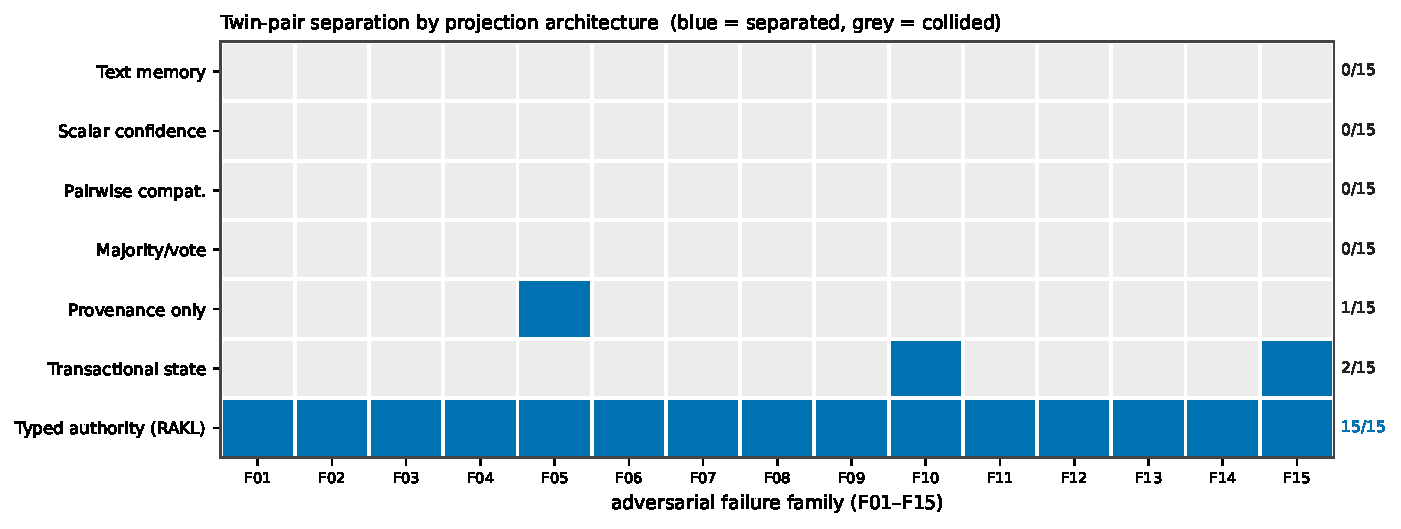
\includegraphics[width=\textwidth]{figures/projection_collision.pdf}
\caption{Twin-pair separation structure behind Table~\ref{tab:projection-sufficiency}. Each cell records whether a projection architecture (rows) separates the minimal twin pair of an adversarial failure family (columns, F01--F15) or collides it; blue is separated, grey is collided. Six representation-level baselines collide on 13--15 of the fifteen families, while only the typed authority projection separates all fifteen. The advantage is therefore a broad structural property of which coordinate each family turns on, not an artefact of a single aggregate score. Computed live from the same audit code as Table~\ref{tab:projection-sufficiency}.}
\label{fig:projection-collision}
\end{figure}

The aggregate numbers are less informative than the collision pattern (Figure~\ref{fig:projection-collision}). The provenance-only representation distinguishes the correlated-versus-independent-root twin because independence is part of that projection, but it still collapses the higher-order-gluing, prediction-versus-mechanism and mechanism-versus-identification twins. The simple transactional state distinguishes the supersession twins because active/version/superseded fields are present, yet it still collapses the typed evidential and causal-authority distinctions. Pairwise compatibility necessarily collapses the parity-style higher-order-gluing twin because pairwise compatibility is fixed while global compatibility changes. The typed projection separates every registered twin because the load-bearing coordinate is retained.

A blanket ``hold'' policy cannot exploit the zero-leakage side of this comparison: it is correct on only 0.367 of the constructed worlds and has zero recall on legitimate canonical changes. The benchmark therefore couples representation sufficiency to non-refusal controls rather than rewarding systems that achieve safety by preventing all scientific state evolution.

\subsection{Interpretation and boundary}

The audit supports a narrow architectural claim. On these registered twins, several plausible compressed states are not sufficient representations for the target update function; their collisions create a nonzero error lower bound before any model or prompt is chosen. Conversely, the typed state is sufficient for this constructed panel. This is not evidence that Orion has learned the hidden coordinate from natural-language science, that the 15 twins exhaust real epistemic failure modes, or that a language model supplied with unrestricted raw observations could not infer a missing fact. Behavioural evaluation of actual proposal systems and natural scientific construct validity remain separate empirical coordinates.

The result nevertheless sharpens the motivation for typed epistemic state. The design question is not whether every scientific distinction deserves a new field. It is whether removing a field causes scientifically distinct states to become observationally identical to the canonical update mechanism. Minimal twins make that question falsifiable: if a simpler projection separates every required action at lower cost, the richer state has not earned its complexity for that scope.
